\scanpage{12}
8°) --- Trouver $U$ ; il suffit encore que $X_{U_0}$ soit ``ess. libre'' sur $U_0$, OK par EGA IV 11

La condition énoncée dans le th. signifie ceci :

$(L)$ Pour tt $T$ spectre d'un anneau de \deleted{valuation discrète} \inserted{local noeth.}, [complet à corps résiduel alg. clos si on y tient, \deleted{\unsure{tout}} \unsure{tels} que $F_T$ sur $X_T/T$ soit plat sur $T$ dans un voisinage de la fibre générique [resp. et $F_{T_0}\ne0$, où $T_0$ le pt fermé\ldots], \deleted{alors} $E_T$ est plat sur $T$, \deleted{\unsure{Exemple}}
\margin{\figure{\begin{tikzpicture}\draw (0,3)..controls(.45,3.2)and(.35,2.9)..(.35,2.2)..controls(.3,1.7)and(.35,1.65)..(.7,1.5)..controls(.32,1.25)and(.32,1.05)..(.3,.5)..controls(.3,.1)and(.2,.1)..(-.2,-.1);\end{tikzpicture}}\uline{N.B.} On peut supposer $\dim T=1$ \deleted{$T$ irréductible} $T$ \unsure{irréduc.|primaire} i.e. $\operatorname{Ass}\underline{O}_T$ réduit à un \unsure{élément|point}, et $T_{\mathrm{réd}}$ Spec d'un anneau de valuation discrète\ldots}

\uline{Corollaire 1} O.K. si $f:X-S$ est \uline{propre}.

\uline{Corollaire 2} O.K. si \deleted{$\unsure{G}$} $F=\underline{O}_X$, $X$ un préschéma \uline{en groupes} sur $S$, satisfaisant la condition $R$ plus haut ---

\uline{Corollaire 3} Soit $f:X\longrightarrow S$ un morphisme de \deleted{type fini, $S$ loc. noeth.} \inserted{prés. finie}. Conditions équivalentes

(i) $f$ se factorise en $f'f''$ : \inserted{\deleted{$X\longrightarrow\unsure{S'}\longrightarrow S$, $S'$ \unsure{loc. noeth.}}} avec $f''$ fid plat, $f'$ \uuline{imm}

(i bis) \figure{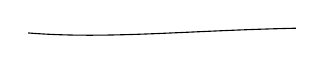
\begin{tikzpicture}[x=1cm,y=1cm]\draw (0,0)..controls(1,-.08)and(2,.03)..(3.4,.06);\end{tikzpicture}} avec $f''$ plat, $f'$ \unsure{imm|mono},

(ii) $\unsure{\varphi_2|p_2}$ de $X\times_S X\xrightarrow{\mathrm{pr}_1}X$ est \uline{plat}
\figure{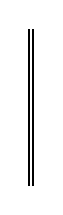
\begin{tikzpicture}[x=1cm,y=1cm]\draw[line width=.7pt](0,0)--(0,2);\draw[line width=.7pt](.06,0)--(.06,2);\end{tikzpicture}}
\mspage{11}
